\documentclass[border=12pt,12pt]{standalone}
\usepackage[american]{circuitikz}

\begin{document}
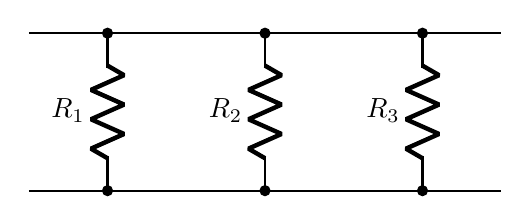
\begin{tikzpicture}[transform shape, scale=1.0,thick]
\ctikzset{bipoles/thickness=2}

%Draw Parallel Resistors
\draw (0, 0) to [R=$R_1$] (0, 2) ;
\draw (2,0) to [R = $R_2$] (2, 2);
\draw (4,0) to [R = $R_3$] (4, 2);

%Draw Lower Line
\draw (-1,0) to [short,-*] (0,0);
\draw (0,0) to [short,-*] (2,0);
\draw (2,0) to [short,-*] (4,0);
\draw (4,0) to [short,-] (5,0);

%Draw Upper Line
\draw (-1,2) to [short,-*] (0,2);
\draw (0,2) to [short,-*] (2,2);
\draw (2,2) to [short,-*] (4,2);
\draw (4,2) to [short,-] (5,2);

\end{tikzpicture}  
\end{document}